\begin{frame}{What is revision control?}
    \begin{itemize}
        \item More commonly known as "Source Control Management" (SCM)
        \pause
        \item Two major types:
        \begin{itemize}
            \item Centralised SCM
            \begin{itemize}
                \item Server: The Repository
                \item Client: Local changes
            \end{itemize}
            \pause
            \item Decentralised SCM
            \begin{itemize}
                \item Anyone can be the server %(GDP)
                \item Complete history
                \item Offline usage
            \end{itemize}
        \end{itemize}  
    \end{itemize}  
\end{frame}

\begin{frame}{Git: A Decentralised SCM}
    \begin{block}{Just remember, you have everything locally}
    \begin{figure}[ht]
        \centering
        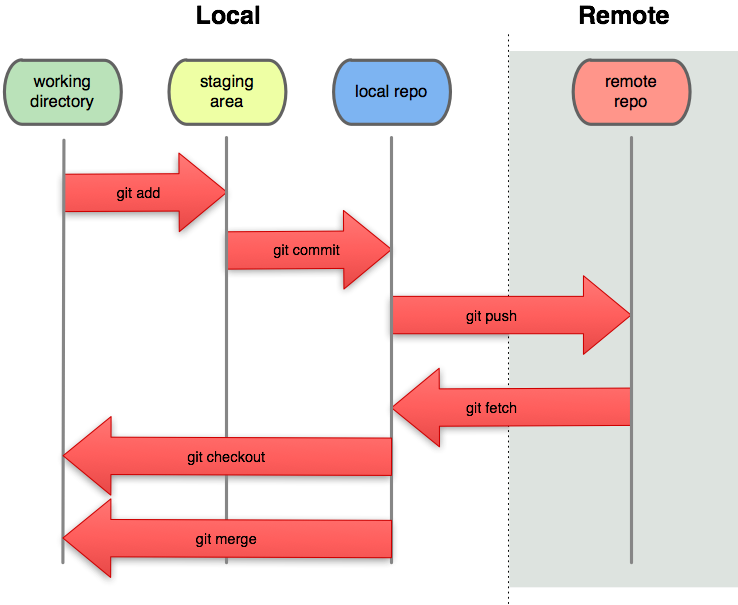
\includegraphics[width=0.6\linewidth]{img/overview.png}
        \caption{Git has several layers allowing for complete control\footnote{Image from \href{http://whygitisbetterthanx.com/}{http://whygitisbetterthanx.com/}}}
        \label{fig:figure0}
    \end{figure}
    \end{block}
\end{frame}

\begin{frame}{Under the hood?}
    \begin{block}{Google it!}
        It can get pretty advanced pretty quickly
    \end{block}
\end{frame}
